\documentclass{beamer}

%% Theme and color scheme
\usetheme{Madrid}
\usecolortheme{default}
\usecolortheme[named=blue]{structure}

%% Packages
\usepackage[utf8]{inputenc}
\usepackage[T1]{fontenc}
\usepackage{amsmath}
\usepackage{amssymb}
\usepackage{graphicx}
\usepackage{subcaption}
\usepackage{xcolor}
\usepackage{tikz}
\usepackage{hyperref}
\usepackage{listings}
\usepackage{verbatim}
\usepackage{booktabs}
\usepackage{multirow}

%% Color definitions for consistency with report theme
\definecolor{lisn-blue}{RGB}{30, 60, 120}
\definecolor{lisn-light}{RGB}{100, 150, 200}
\definecolor{accent-color}{RGB}{200, 50, 50}

\setbeamercolor{structure}{fg=lisn-blue}
\setbeamercolor{background canvas}{bg=white}

%% Listings configuration
\lstset{
    basicstyle=\ttfamily\small,
    keywordstyle=\color{blue},
    commentstyle=\color{gray!60},
    stringstyle=\color{green!60!black},
    breaklines=true,
    frame=single,
    backgroundcolor=\color{gray!5}
}

%% Title slide information
\title{Blob Computing in Homogeneous Isotropic Distributed Systems}
\author{Lucas Labouret}
\institute{
    Université Paris-Saclay \\[0.3cm]
    \textit{Performed at}\\
    Laboratoire Interdisciplinaire des Sciences du Numériques (LISN) \\[0.3cm]
    \textit{Supervised by}\\ 
    Frédéric Gruau
}
\date{September 2nd, 2026}

%% Footer with slide numbers and author
\setbeamertemplate{footline}{%
    \hbox{
        \begin{beamercolorbox}[wd=0.66\paperwidth,ht=2.25ex,dp=1ex,center]{title in head/foot}%
            \insertshorttitle
        \end{beamercolorbox}%
        \begin{beamercolorbox}[wd=0.33\paperwidth,ht=2.25ex,dp=1ex,right]{date in head/foot}%
            \insertframenumber{} / \inserttotalframenumber\hspace*{2ex}
        \end{beamercolorbox}%
    }%
    \vskip0pt%
}

%% Customize itemize bullets
\setbeamertemplate{itemize items}[circle]
\setbeamercolor{itemize item}{fg=lisn-blue}

\begin{document}

\begin{frame}[plain]
    \titlepage
    \vfill
    \begin{center}
        \small Master 2 Quantum and Distributed Computer Science (QDCS) \\
        2025-26 Internship Defense
    \end{center}
\end{frame}

\section*{Outline}
\begin{frame}{Outline}
    \tableofcontents
\end{frame}

\section{Introduction}

\begin{frame}{Context: Moore's Law Reaching Its Limits}
    \begin{itemize}
        \item Current trend: transistor miniaturization increases computational power.
        \item Recent achievement: IBM's 0.7nm nodes (roughly 15 rows of silicon atoms).
        \item Challenge: approaching physical limits of miniaturization.
        \item Solution: scale up computationally by increasing the area of chips.
    \end{itemize}
    \vfill
    \begin{center}
        \textbf{Current paradigm do not take physical distance into account, and tend not to scale well with increasing size.}
    \end{center}
\end{frame}

\begin{frame}{Host Organization}
    \textbf{LISN - Laboratoire Interdisciplinaire des Sciences du Numériques}
    \begin{itemize}
        \item Located in Orsay
        \item Part of Université Paris-Saclay and CNRS
    \end{itemize}
    
    \vfill

    \textbf{Supervisor: Frédéric Gruau}
    \begin{itemize}
        \item Associate Professor
        \item Expertise: Cellular automata \& Natural computing
    \end{itemize}
\end{frame}

\begin{frame}{Performed Work}
    \begin{enumerate}
        \item \textbf{Defined a Blob language} and implemented an interpreter
            \begin{itemize}
                \item Reuse parallel simulation techniques from M1 internship
            \end{itemize}
    
    \vfill

        \item \textbf{Developed a graphical user interface}
            \begin{itemize}
                \item Visualize Blob program execution
                \item Enable interaction with simulation
            \end{itemize}
        
    \vfill

        \item \textbf{Started designing an algorithm for the homogenization problem}
            \begin{itemize}
                \item Related to load balancing in distributed systems
                \item Self-organization using only local information
                \item Still ongoing work, but preliminary results are promising
            \end{itemize}
    \end{enumerate}
\end{frame}

\section{Blob Computing Paradigm}

\begin{frame}{What is Blob Computing?}
    \begin{block}{Definition}
        A massively parallel computational paradigm based on:
        \begin{itemize}
            \item Interactions of simple, locally communicating processing elements (PEs).
            \item Spatial arrangement of processing elements.
            \item Information propagation time scales linearly with distance.
        \end{itemize}
    \end{block}
    
    \pause

    \begin{block}{Key Advantage}
        Individual PEs quickly disappear from the programmer's perspective in favor of \textbf{Blobs}, which are connected groups of PEs treated as single units.
    \end{block}

    \pause
    
    \begin{block}{Objective}
        Achieve arbitrarily scalable computational power by simply increasing the number of PEs in the system
    \end{block}
\end{frame}

\begin{frame}{Current Status}
    \begin{center}
        \Large \textbf{Internship Timeline}
    \end{center}
    
    \vspace{1cm}
    
    \begin{itemize}
        \item Defense scheduled: September 2nd, 2025
        \item Internship completion: October 23rd, 2025
        \item Status: $\approx$ 75\% of time remaining after defense
    \end{itemize}
    
    \vspace{1cm}
    
    \begin{alertblock}{Note}
        Information in this presentation is subject to change as work continues on the project
    \end{alertblock}
\end{frame}


\begin{frame}{Blob Computing at the Micro Level}
    PEs
    \begin{itemize}
        \item execute the same sequence of instructions synchronously
        \item are arranged according to a Delaunay triangulated planar graph
        \item communicate only with their immediate neighbors, and cannot distinguish between neighbors of the same type
        \item have no knowledge of their position, nor of the graph's structure
        \item are anonymous
        \item agree on a common orientation, but not on a common direction
    \end{itemize}
\end{frame}

\begin{frame}{Computing Medium Structure}
    \begin{figure}[h]
        \centering
        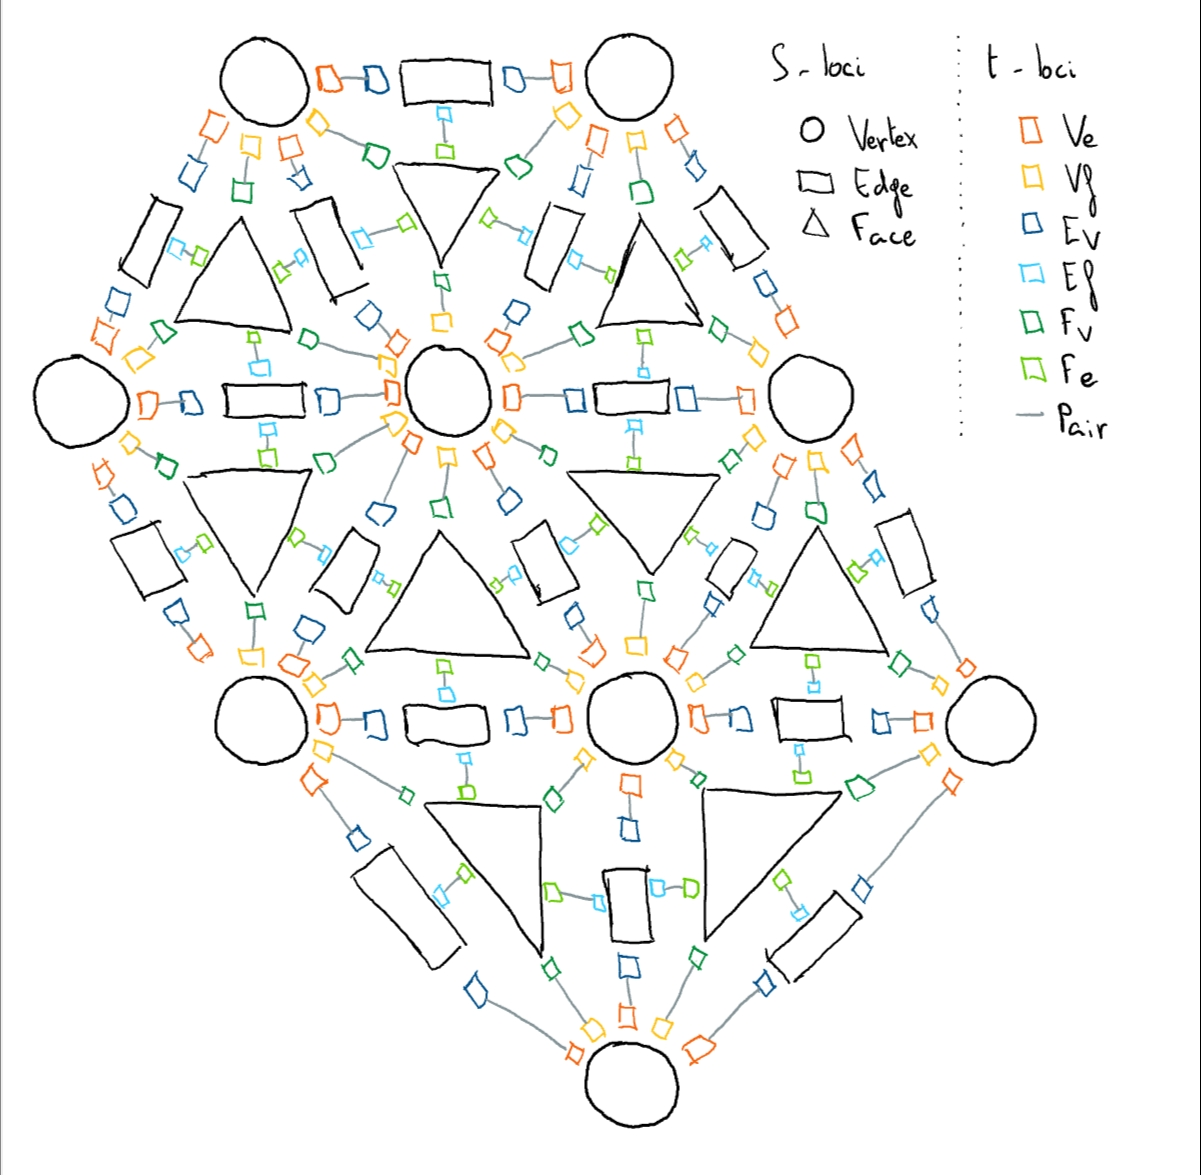
\includegraphics[width=0.6\textwidth]{figs/handdrawn_medium.png}
        \caption{A simple example of a computing medium}
    \end{figure}
\end{frame}

\begin{frame}{Computing Medium Structure}
    \begin{figure}
        \centering
        \begin{subfigure}{.45\textwidth}
            \centering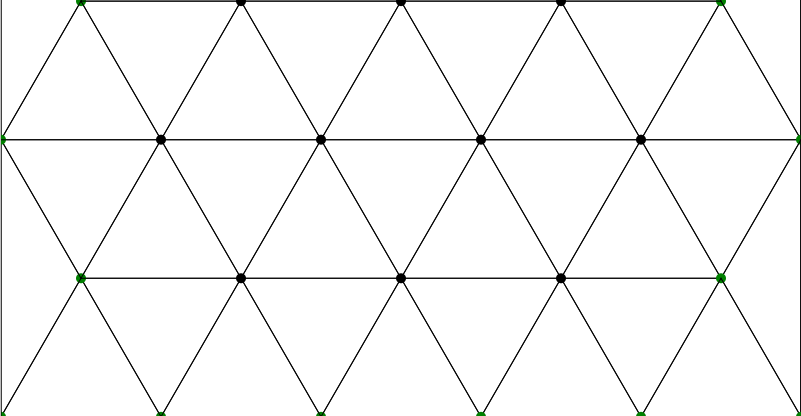
\includegraphics[width=\linewidth]{figs/medium_homogeneous.png}
            \caption{Homogeneous but not isotropic.}
        \end{subfigure}
        \begin{subfigure}{.45\textwidth}
            \centering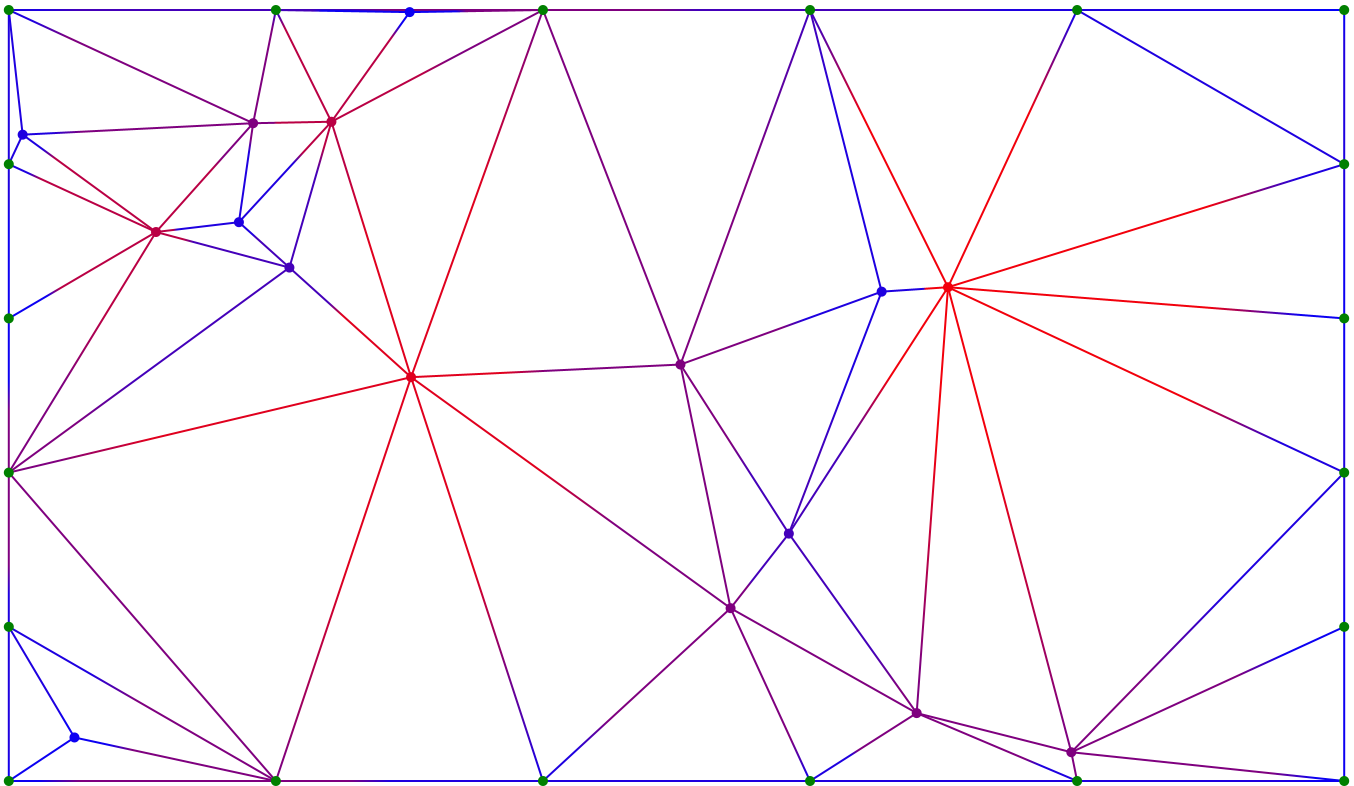
\includegraphics[width=\linewidth]{figs/medium_isotropic.png}
            \caption{Isotropic but not homogeneous.}
        \end{subfigure}
        \begin{subfigure}{.45\textwidth}
            \centering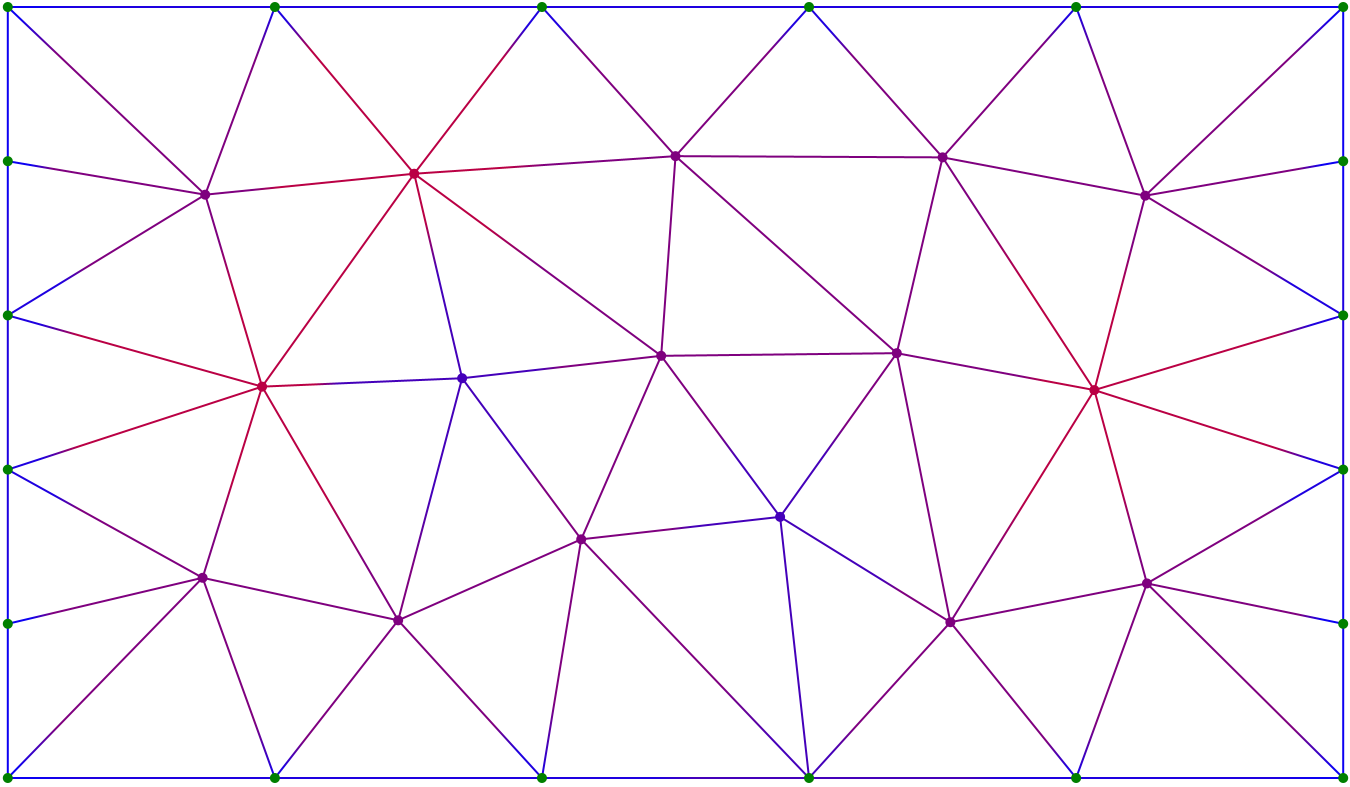
\includegraphics[width=\linewidth]{figs/medium_homogeneous_isotropic.png}
            \caption{Homogeneous and isotropic.}
        \end{subfigure}
    \end{figure}
\end{frame}

\begin{frame}{Most used medium}
    \begin{figure}
        \centering
        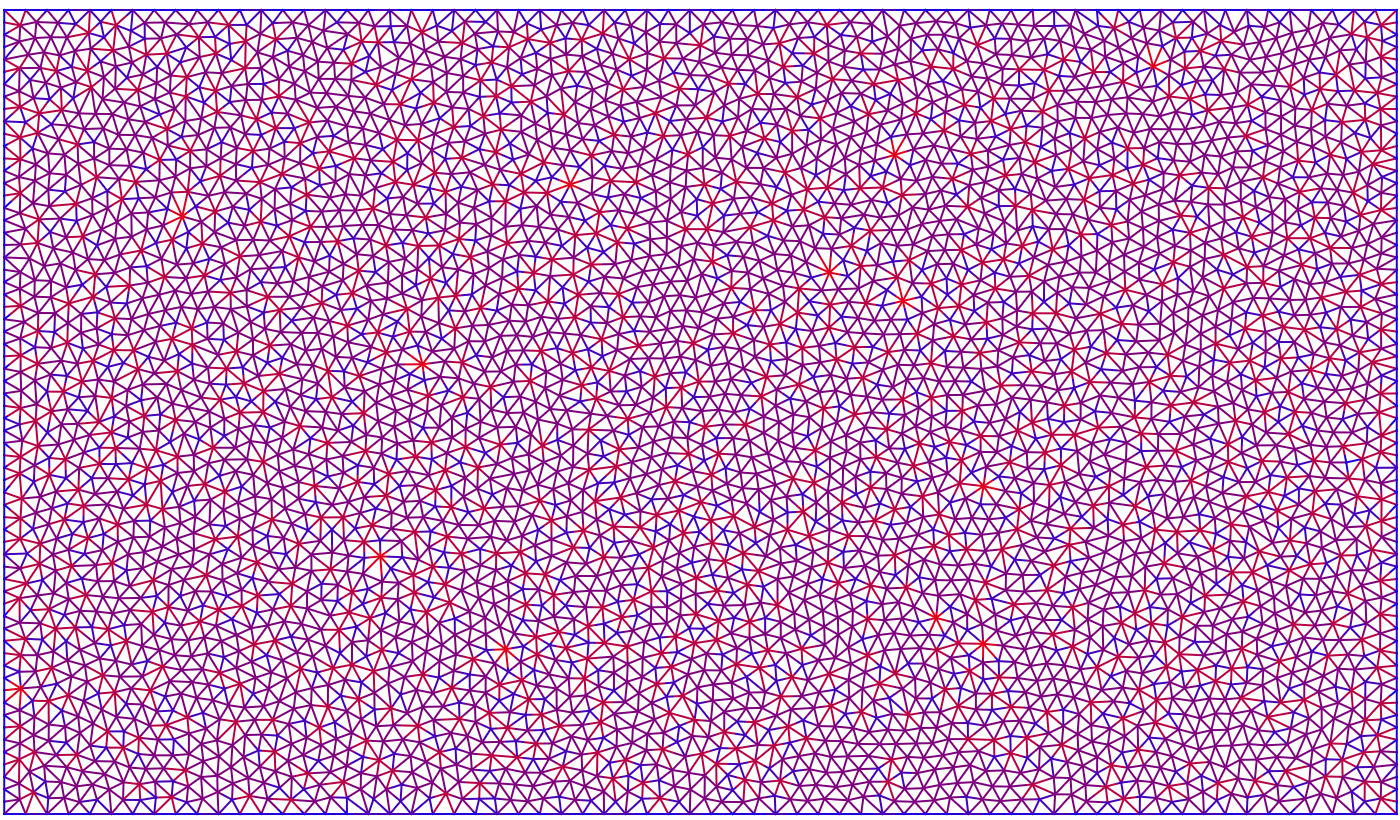
\includegraphics[width=0.9\textwidth]{figs/large_medium.png}
        \caption{Homogeneous isotropic medium with 4355 vertices.}
    \end{figure}
\end{frame}

\section{Blobs and Fields}

\begin{frame}{Blobs and Fields}
    \label{voronoi}
    \begin{figure}[ht]
    \centering
    \begin{subfigure}{0.3\textwidth}
        \centering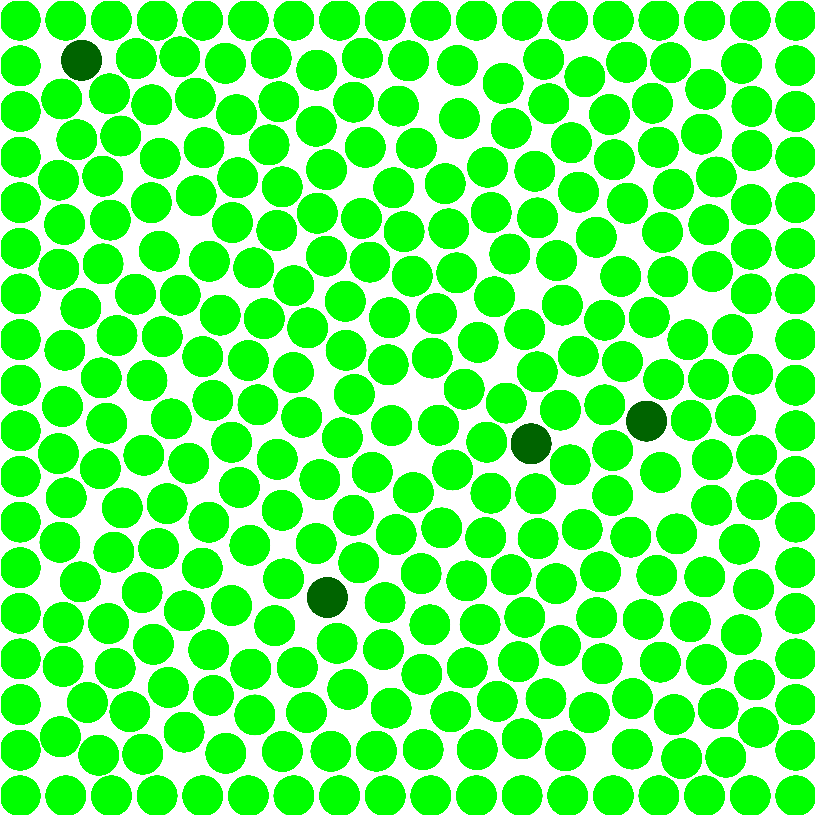
\includegraphics[width=\linewidth]{figs/static_voronoi_0.png}
    \end{subfigure}
    \begin{subfigure}{0.3\textwidth}
        \centering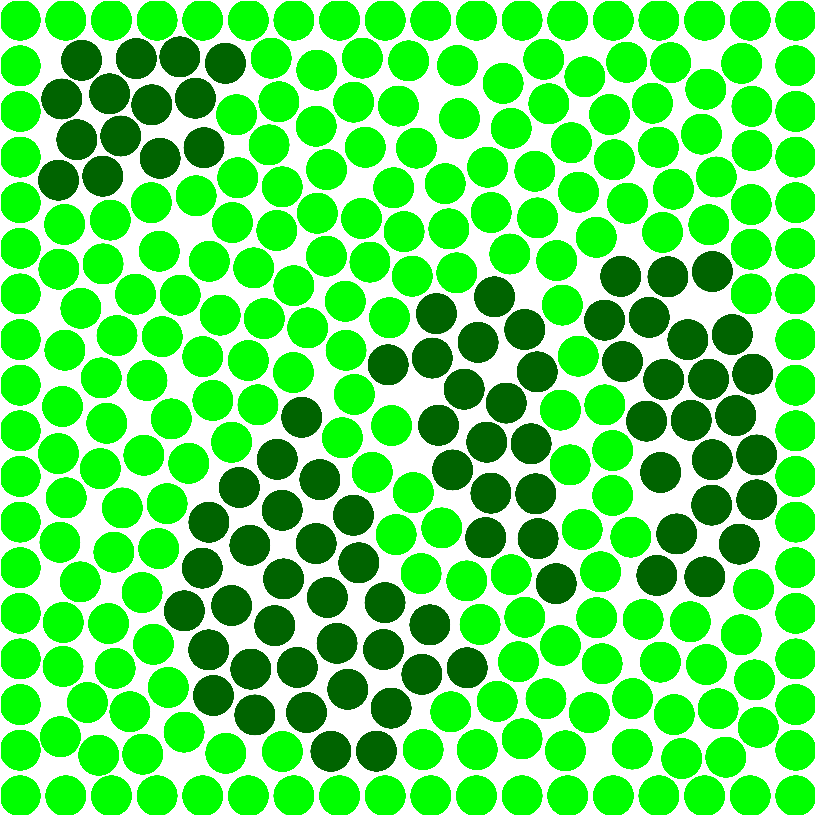
\includegraphics[width=\linewidth]{figs/static_voronoi_1.png}
    \end{subfigure}
    \begin{subfigure}{0.3\textwidth}
        \centering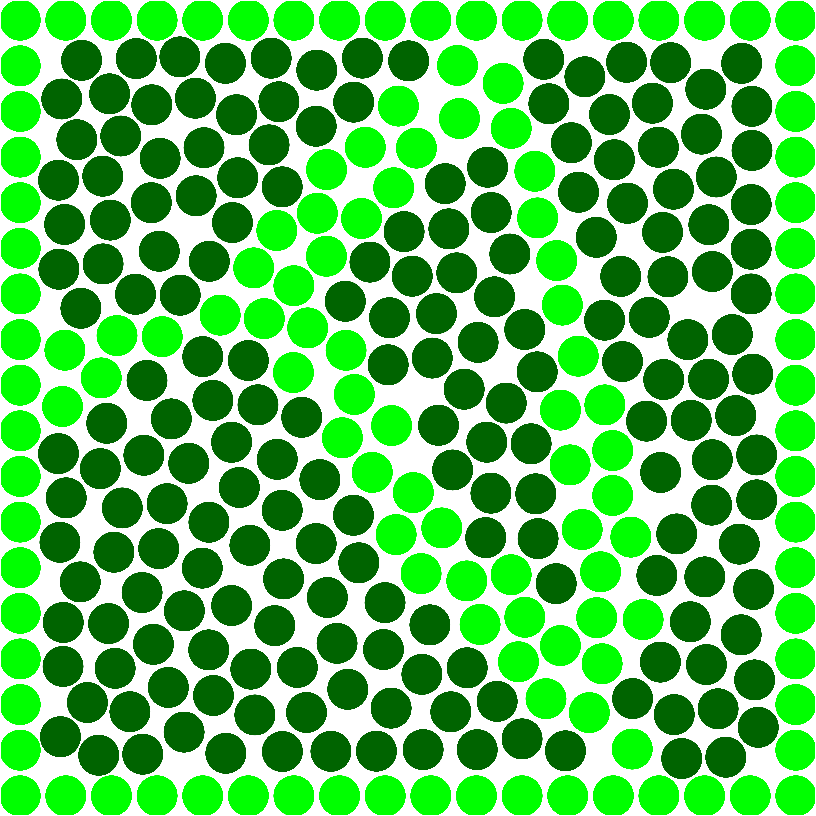
\includegraphics[width=\linewidth]{figs/static_voronoi_2.png}
    \end{subfigure}
    \caption{\centering Construction of the Voronoï computation of 4 static particles in a medium.}
\end{figure}
\end{frame}

\section{Language, Interpreter and GUI}

\begin{frame}{Blob Language and Interpreter}
    \textbf{Language}: Built on top of Java to reduce development time
    \begin{itemize}
        \item Leverages Java's existing features :
            \begin{itemize}
                \item Object-oriented programming
                \item Strong typing
                \item Exception handling
                \item ...
            \end{itemize}
        \item Skips the need to implement basic language features from scratch such as lexical analysis, parsing, type checking, etc.
    \end{itemize}

    Interesting features:
    \begin{itemize}
        \item Fully object-oriented
        \item Slight metaprogramming capabilities
        \item Many errors are caught before execution, during the construction of the instruction sequence
    \end{itemize}
\end{frame}

\begin{frame}{GUI}
    \begin{figure}[ht]
    \centering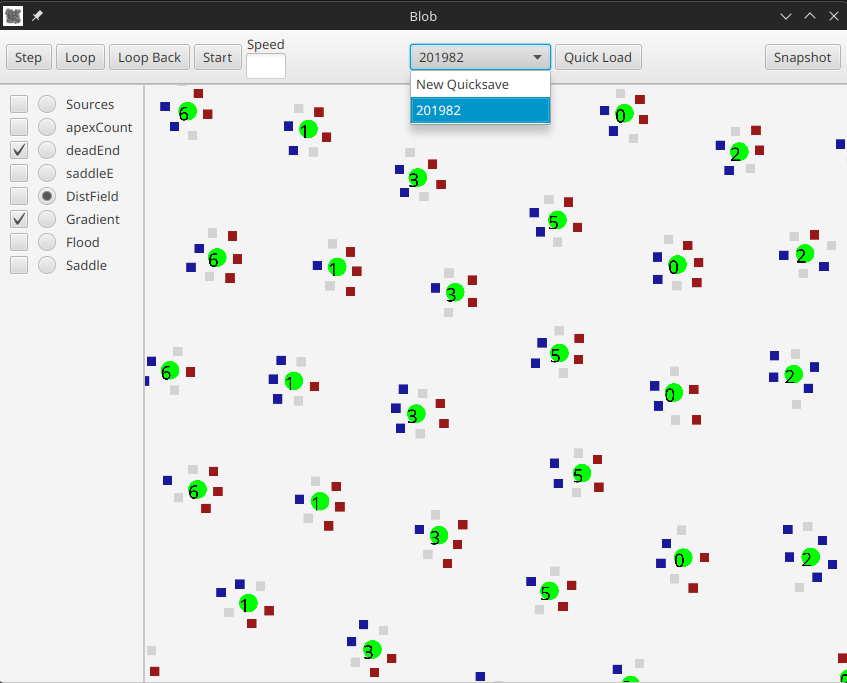
\includegraphics[width=0.7\linewidth]{figs/main_interface.png}
\end{figure}
\end{frame}

\section{Homogenization Problem}

\begin{frame}{Homogenization Problem Definition}
    \begin{definition}
        \textbf{Homogenization}: Given a set of particles distributed in a computing medium, the goal is to rearrange them so as to \textbf{maximize the minimum distance} between any two particles.
    \end{definition}

    \begin{itemize}
        \item \textbf{Practical relevance}
            \begin{itemize}
                \item Similar to load balancing
                \item Well-fitted to Blob computing due to its spatial nature
            \end{itemize}
        
        \item \textbf{Research opportunity}
            \begin{itemize}
                \item Self-organization problem
                \item Rather complex but solved for the crystalline lattice
            \end{itemize}
    \end{itemize}
\end{frame}

\begin{frame}{Planned Approach}
    \begin{enumerate}
        \item Compute the distance field of the particles
        \item Determine the Gabriel centers of the set of particles
        \item Build the Vornoi diagram of the particles based on the Gabriel centers
        \item Move each particle toward the center of its Vornoi cell
    \end{enumerate}

    \vfill

    \begin{block}{Note}
        Because the particles are moving, we cannot reuse the Voronoï construction of slide \ref{voronoi}.
    \end{block}
\end{frame}

\begin{frame}{Distance Field}
    \begin{figure}
        \centering
        \begin{subfigure}{0.8\linewidth}
            \centering
\includegraphics[width=\linewidth]{figs/distance_distance.png}
            \caption{Distance field.}
        \end{subfigure}
        \begin{subfigure}{0.8\linewidth}
            \centering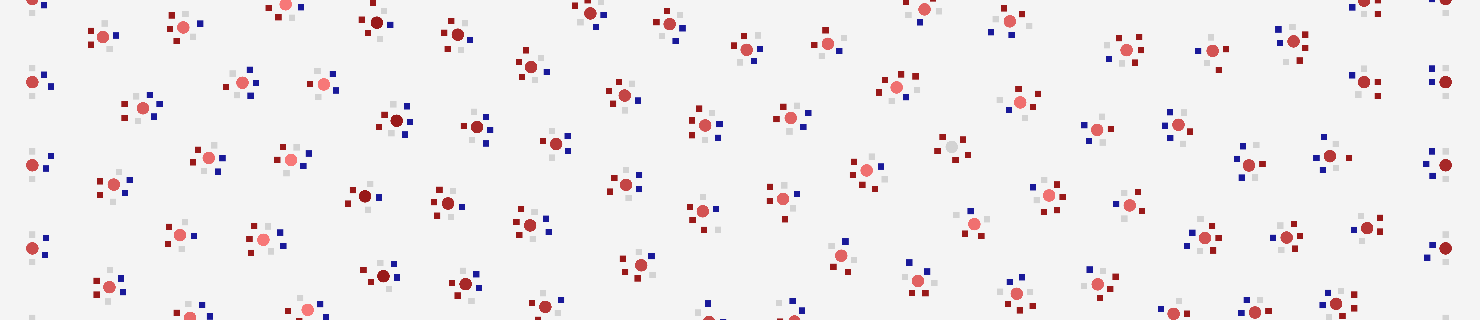
\includegraphics[width=\linewidth]{figs/distance_gradient.png}
            \caption{Gradient field.}
        \end{subfigure}
    \end{figure}
\end{frame}

\begin{frame}{Gabriel Centers}
    \begin{figure}
        \centering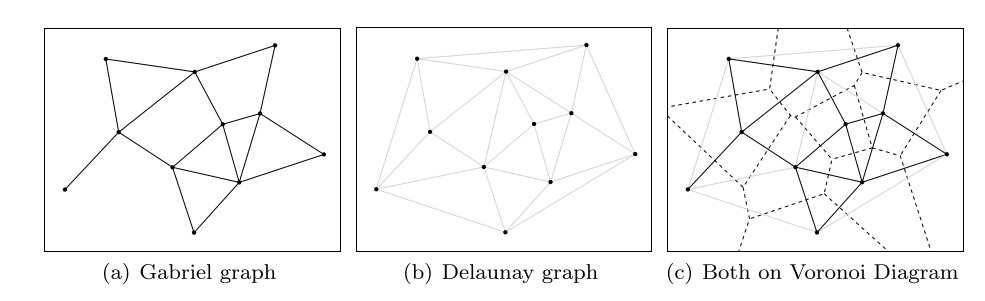
\includegraphics[width=\linewidth]{figs/gabriel_centers.jpeg}
    \end{figure}

    \vfill

    \begin{block}{Hexagonal lattice}
        The Gabriel centers are the vertices or edges where the gradient field descend in multiple distinct directions.
    \end{block}

    \begin{alertblock}{}
        Isotropy introduces erroneous detections.
    \end{alertblock}
\end{frame}

\begin{frame}{Method 1: Error Correction}
    \begin{figure}
        \centering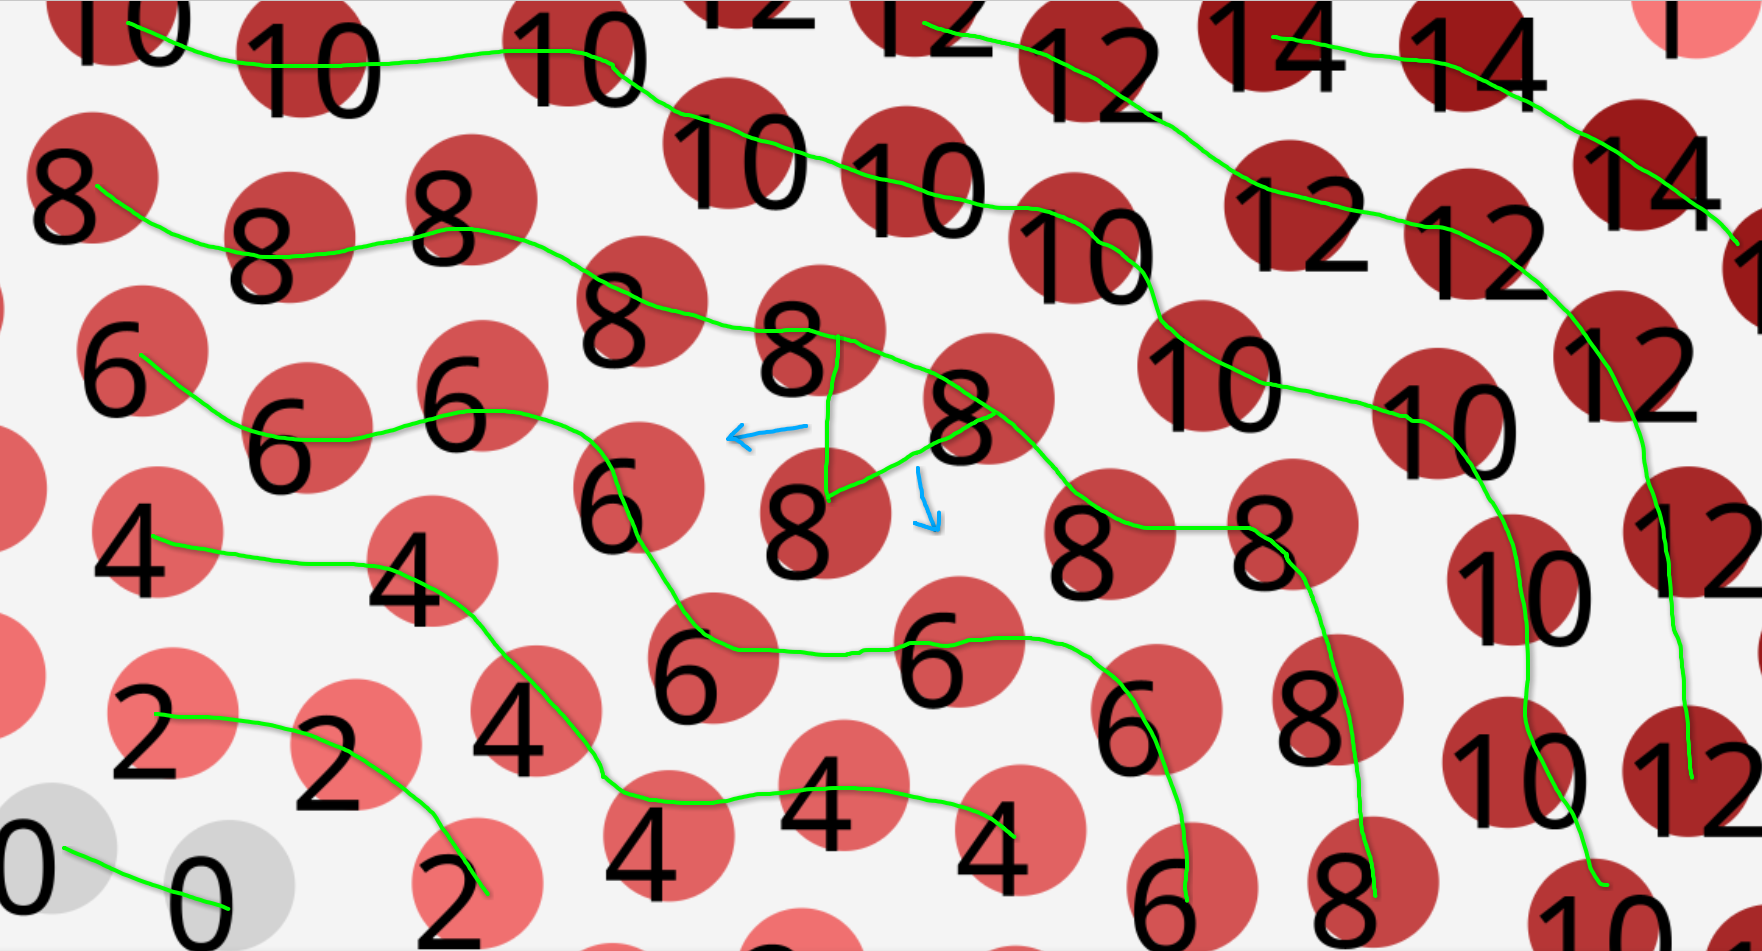
\includegraphics[width=\linewidth]{figs/split_plateau.png}
        \caption{An erroneous detection.}
    \end{figure}
\end{frame}

\begin{frame}{Method 2: Flooding}
    \begin{figure}
    \centering
    \begin{subfigure}{0.42\linewidth}
        \centering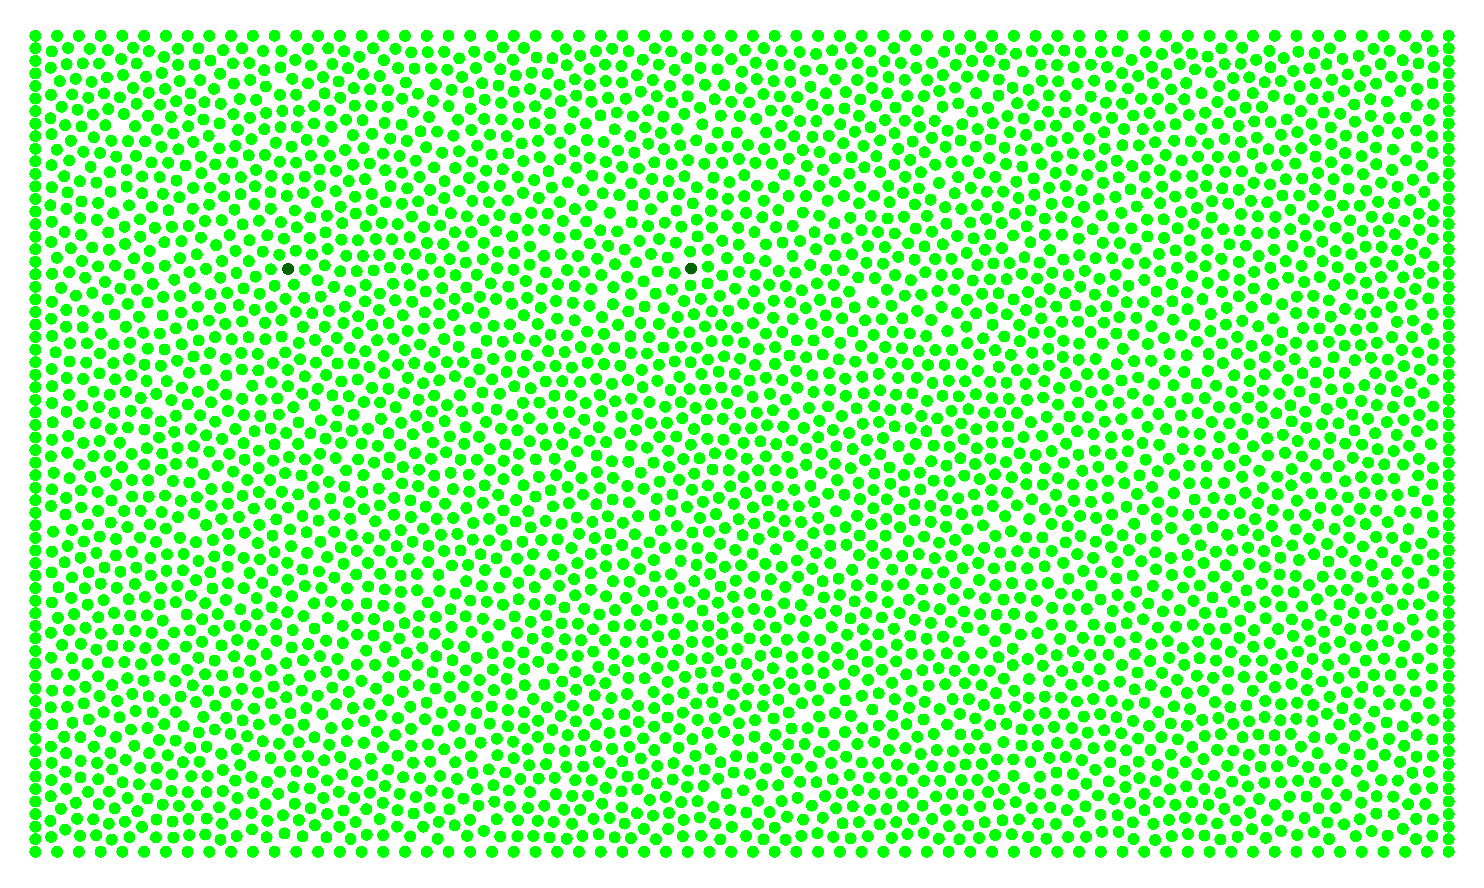
\includegraphics[width=\linewidth]{figs/flooding_particles.png}
        \caption{The set of particles.}
    \end{subfigure}
    \begin{subfigure}{0.42\linewidth}
        \centering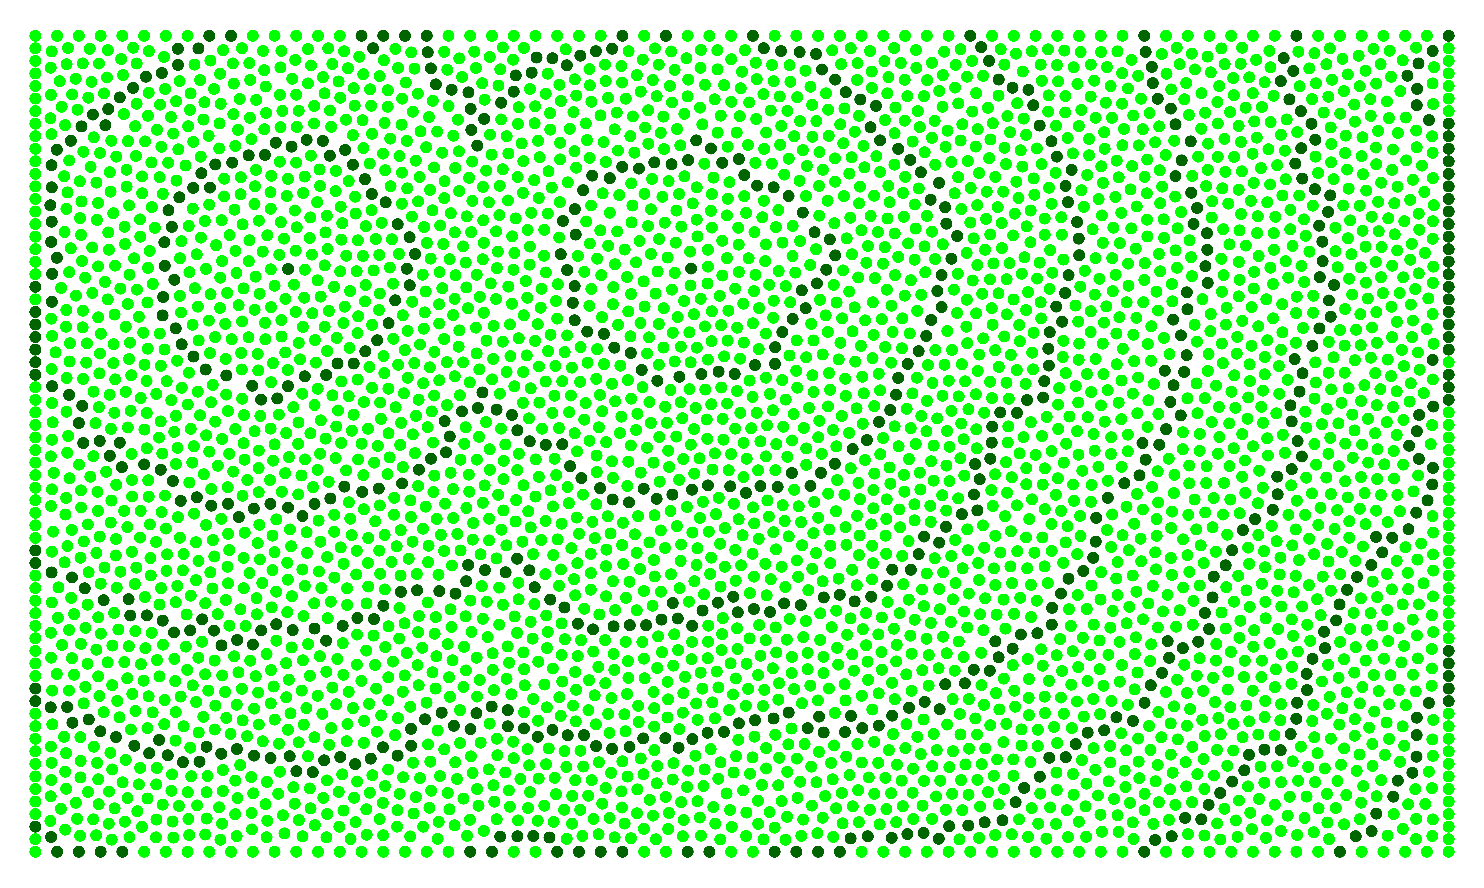
\includegraphics[width=\linewidth]{figs/flooding_starting_points.png}
        \caption{The starting points of the floods.}
    \end{subfigure}
    \begin{subfigure}{0.42\linewidth}
        \centering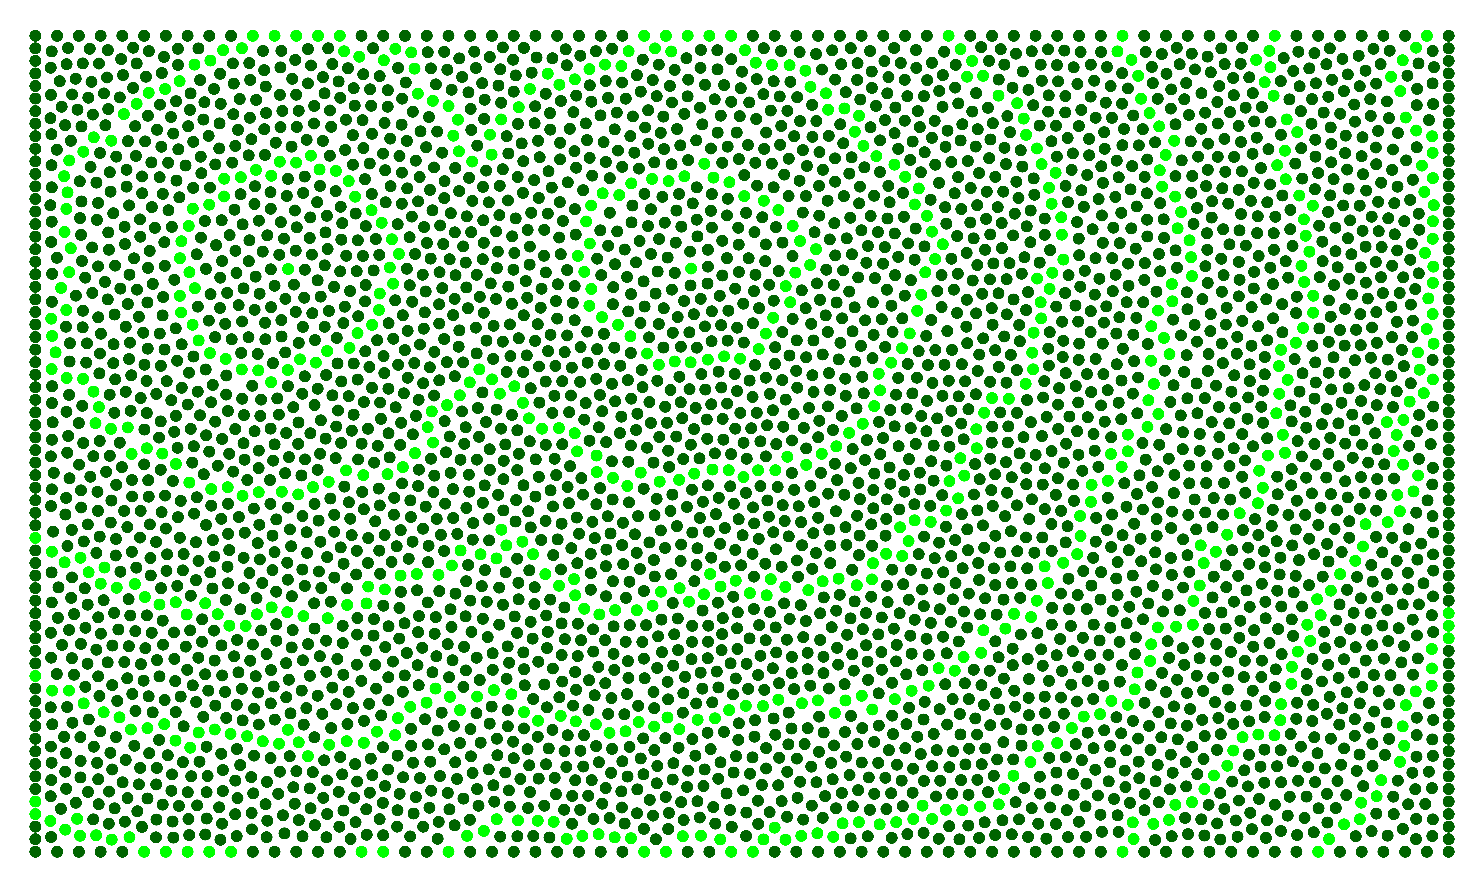
\includegraphics[width=\linewidth]{figs/flooding_flood.png}
        \caption{The flooding of the medium.}
    \end{subfigure}
    \begin{subfigure}{0.42\linewidth}
        \centering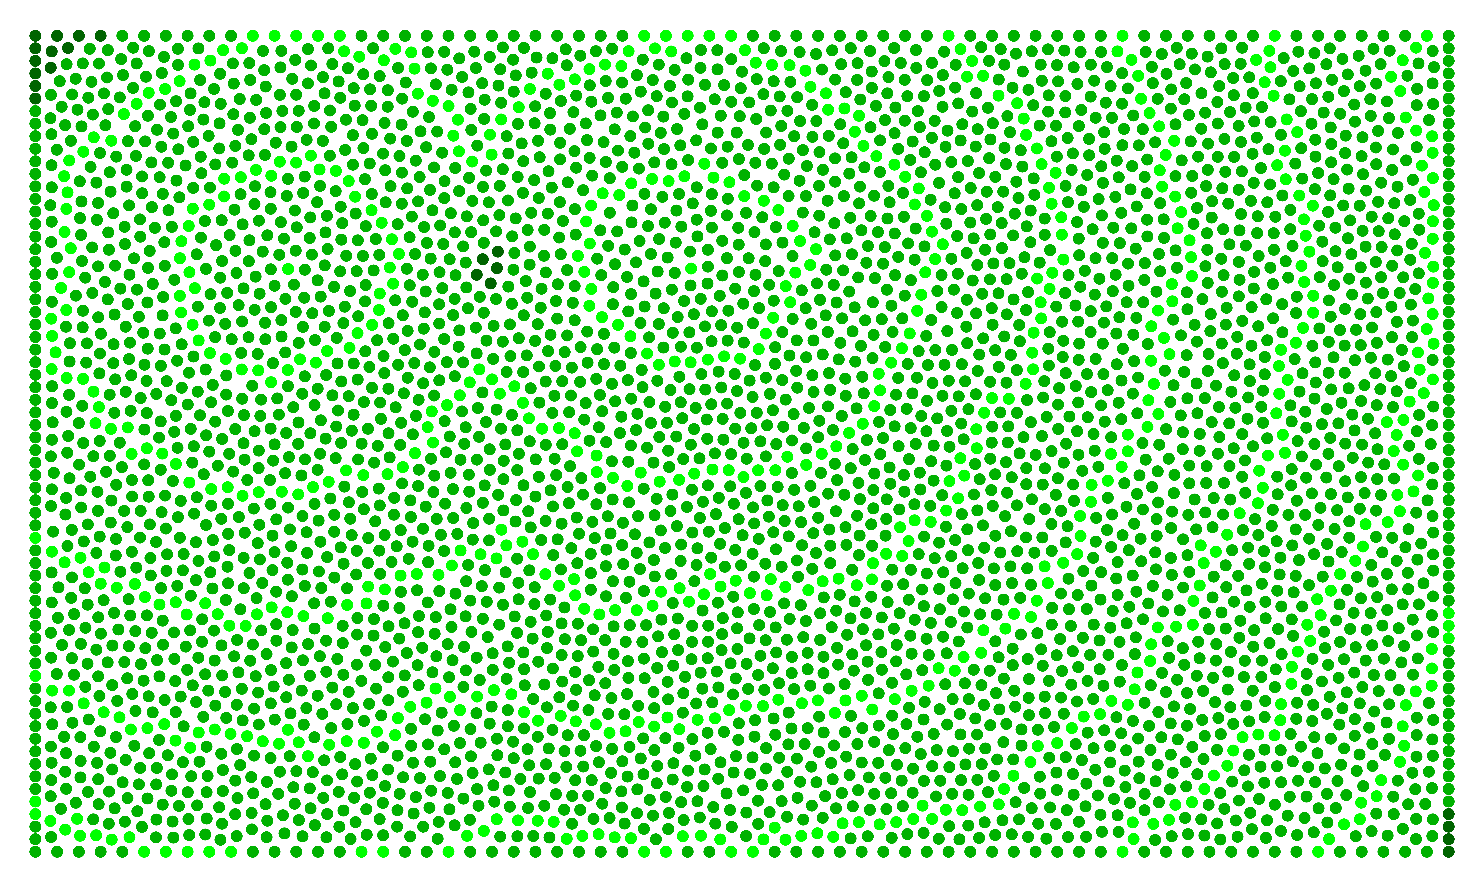
\includegraphics[width=\linewidth]{figs/flooding_centers.png}
        \caption{The detected Gabriel centers.}
    \end{subfigure}
    \label{fig:flood}
\end{figure}
\end{frame}

\section{Conclusion}

\begin{frame}{Repercussions of the Work}
    Technical contributions:
    \begin{itemize}
        \item Blob language and interpreter
        \item GUI for visualizing and interacting with Blob programs
        \item Preliminary results on homogenization problem
    \end{itemize}
    
    \vfill    

    Personal impact:
    \begin{itemize}
        \item Gained experience in software development and GUI design
        \item Furthered my understanding of distributed computing and parallel programming
        \item Improved my problem-solving and research skills
        \item Confirmed my interest in pursuing a career in research and development
    \end{itemize}
\end{frame}

\section{Resources}

\begin{frame}{Project Repository}
    \begin{center}
        Code available at:
        
        \vspace{0.5cm}
        
        \texttt{\url{https://github.com/Lucas-Labouret/BlobComputing}}
    \end{center}
\end{frame}

\begin{frame}[plain]
    \begin{center}
        \Large
        \textbf{Thank you for your attention!}
        
        \vspace{2cm}
        
        \normalsize
        Contact: \texttt{lucas.labouret@universite-paris-saclay.fr}
        
        \vspace{1cm}
        
        LISN, Université Paris-Saclay
    \end{center}
\end{frame}

\end{document}
